%!TeX spellcheck = en_UK
% Die erste (unkommentierte) Zeile im Dokument legt immer die
% Dokumentklasse fest
\documentclass{scrartcl} 

% Präambel:
% Einbinen von zusätzlichen Paketen. Falls für eine Datei keine Endung
% explizit angegeben wird, benutzt LaTeX '.tex'. Im Folgenden wird
% also die Datei 'edv_pakete.tex' eingebunden.
% Die erste Zeile im Dokument legt immer die Dokumentklasse fest
%\documentclass[notitlepage]{scrreprt}
    % Die wichtigsten Dokumentklassen:
    %   scrbook, scrreprt, scrartcl, beamer, standalone
    % Einige gängige Optionen für \documentclass:
    %   ngerman
    %   titlepage, notitlepage
    %   onecolumn, twocolumn
    %   oneside, twoside
    %wird in Hauptdatei festgelegt

% Präambel

% Einige KOMA-Script-Optionen
\KOMAoptions{fontsize=12pt,paper=a4}      %Schriftgröße, Papierformat
\KOMAoptions{DIV=11}                      % Parameter mit dem man den Seitenrand ändern kann
\KOMAoptions{listof=totoc}

% Hier werden einige Pakete eingebunden
\usepackage[utf8]{inputenc}               % Direkte Eingabe von ä usw. Input=Eingabe
\usepackage[T1]{fontenc}                  % Font Kodierung für die Ausgabe Font=Ausgabe
\usepackage[english]{babel}               % Verschiedenste sprach-spezifische Extras, ngerman für neue deutsche Rechtschreibung, auch UK oder US möglich
\usepackage[autostyle=true]{csquotes}     % Intelligente Anführungszeichen, arbeitet mit Babel zusammen
%

\usepackage{amsmath}%Mathedarstellung
\usepackage{commath}%Mathedarstellung
\usepackage{physics}%Physik-Symbole
%\usepackage{IEEEtrantools}%IEEEeqnarray
%
\usepackage{siunitx}   % Intelligentes Setzen von Zahlen und Einheiten
%\sisetup{locale = DE}  % Deutsch als locale für die Zahlen und Einheiten
%http://tex.stackexchange.com/questions/2291/how-do-i-change-the-enumerate-list-format-to-use-letters-instead-of-the-defaul

\usepackage{enumitem}%erlaubt u.A. die Aufzählung mit Buchstaben, gefunden auf http://tex.stackexchange.com/questions/2291/how-do-i-change-the-enumerate-list-format-to-use-letters-instead-of-the-defaul
%
\usepackage[varg]{txfonts}                % Schönere Schriftart, muss nach amsmath, damit keine Fehlermeldung kommt
\usepackage{graphicx} %einbinden von Figuren/Bildern
\graphicspath{{figs/}} % Stammverzeichnis der verwendeten Bilder, muss im selben Ordner wie Hauptdatei sein
%
\usepackage[backend=biber, style=numeric, sorting=none]{biblatex}
%Verwenden von \cite in \footnote: Bibliographie drucken lassen, mehrmals kompilieren
\usepackage{hyperref}%erzeugt klickbare Elemente
\usepackage[all]{hypcap}%hyperref-befehle springen zum oberen Rand des Bildes
% Zum Einbinden von Programmcode verwenden wir das listings-Paket
\usepackage{listings}

% Für Syntax-Highlighting:
\usepackage{xcolor}

\usepackage{longtable}

% Die folgenden listings-Einstellungen sind nötig, um
% deutsche Umlaute und die Tilde (~) in listings-Umgebungen
% verwenden zu können.
\lstset{
    basicstyle=\ttfamily,    
    literate={~} {$\sim$}{1} % set tilde as a literal
    {ö}{{\"o}}1
    {ä}{{\"a}}1
    {ü}{{\"u}}1
    {ß}{{\ss}}1
    {Ö}{{\"O}}1
    {Ä}{{\"A}}1
    {Ü}{{\"U}}1
}

% Farben für Code-Syntaxhighlighting und Weiteres festlegen:
\lstset{
    % Keine besondere Markierung für Leerzeichen in Codes
    showspaces=false,               
    showstringspaces=false,         
    % Farebn für Code-Kommentare und Schlüsselworte:
    commentstyle=\color{red},       % comment style
    keywordstyle=\color{blue},      % keyword style
    stringstyle=\color{orange},		% string style
    breaklines=true,
    numbers=left,                    % where to put the line-numbers; possible values are (none, left, right)
    numbersep=5pt,                   % how far the line-numbers are from the code
    stepnumber=5, 					%how often there are line numbers in code listings
    tabsize=4, 						%default tabsize set to 4 spaces
    %language=python,
    }
%gefunden auf https://en.wikibooks.org/wiki/LaTeX/Source_Code_Listings
%eigene Kommandos/Abürzungen
\newcommand{\tb}{\textbackslash}
\newcommand{\txt}{\texttt}
\newcommand{\umt}{u_{(i+i\%2)/2}^{(2a)}}
\newcommand{\utmt}{u_{(i-2+i\%2)/2}^{(2a)}}
\newcommand{\uti}{\tilde{u}_i^{(a)}}
\newcommand{\utio}{\tilde{u}_{i-1}^{(a)}}




% Verzeichnisse mit Abbildungen; kann gestrichen werden,
% falls Sie dies schon in edv_pakete.tex definiert haben:
%\graphicspath{{../report}}

\addbibresource{refs.bib} %Hinzufügen einer Literaturdatenbank aus dem angegebenen Verzeichnis

% Titel, Autor und Datum
\title{Computational Physics}
\subtitle{Exercise 5}
\date{\today}
\author{Christiane Groß, Nico Dichter}

% Jetzt startet das eigentliche Dokument
\begin{document}
	\maketitle
	
\section{Theory}
\subsection{The Gaussian Model}

We want to simulate the Gaussian model with the following hamiltonian that can also be discretized:
\[
H(u)=\int_{0}^{L}\mathrm{d}x\left(\partial{u(x)} \right)^2=\frac{1}{a}\sum_{i=1}^{N}\left(u_i-u_{i-1} \right)^2=H_a(u)
\]

For the discretization, we divide the length $L$ into $N$ pieces, each of which has length $a=L/N$. This give us $N+1$ points connecting the pieces to the end and to each other. 

We assume Dirichlet-boundary conditions, i.\! e.\! $u(0)=u(L)=0=u_0=u_N$.

Any observable can be calculated the usual way as: \[
\langle O\rangle=\frac{1}{Z}\prod_{i=1}^{N-1}\int\mathrm{d}u_i O(u)\exp(-\beta H(u)) \]
\[
Z=\prod_{i=1}^{N-1}\int\mathrm{d}u_i\exp(-\beta H(u)) 
\]

We set $\beta=1$ and ignore it.

For the multigrid algorithm, we also need a generalized hamiltonian that takes into accout an external field:
\[
H_a(u^{(a)})=\frac{1}{a}\sum_{i=1}^N
\left( u_i^{(a)}-u_{i-1}^{(a)}\right) ^2+a\sum_{i=1}^{N-1}\phi_i^{(a)}u_i^{(a)}
\]

When performing the simulation, we generate new states by selecting a random site, proposing a change $\Delta$ with $\Delta\sim\mathcal{U}[-\delta, \delta]$ and accepting it with probability $\min(1, \exp(H(u)-H(u')))$. By doing this $N-1$ times, we perform one sweep.

We are interested in measuring the average energy, $\langle H\rangle$, as well as the average magnetisation $\langle m \rangle$ and ist square $\langle m^2\rangle$, with $m=\frac{a}{L}\sum_{k=1}^{N-1}u_k$.

\subsection{Multigrid Algorithms}

We are interested in the behaviour of the system for small $a$ and large $N$, but simulating this is expensive in terms of computation time. The multigrid algorithm tries to solve this problem by doing most of the calculation at a coarser level and using these results for interpolating the finer levels.
We first do $\nu$ presweeps at the current level, then, if we aren't at the highest level yet, we do $\gamma$ multigrid sweeps at the next coarsest level, and then do $\nu$ postsweeps.

\paragraph{restrictions}
To be able to do sweeps at a coarser level, we need to determine the Hamiltonian and the lattice $u$ at that level. The derivation of the Hamiltonian is done in section~\ref{subsec:phi2a}, and we do the restriction of $u$ by taking every second grid point: $u_i^{(2a)}=u_{2i}^{(a)}$.

\paragraph{prolongations}
After the sweep at the coarser level, we need to add these results to the finer level. We do this by setting:\[
I^{(a)}_{(2a)}=\begin{cases}
u_{i/2}^{(2a)}& \text{i even}\\
\frac{1}{2}\left(u_{(i-1)/2}^{(2a)}u_{(i+1)/2}^{(2a)}\right) & \text{i odd}\\
\end{cases}
\]

and get our new field by setting $u_i^{(a)}=\tilde{u}_i^{(a)}+(I_{2a}^au^{(2a)})_i$.

\section{Deliberations}

\subsection{analytical solutions}
We were not able to calculate the expactation values of our observables analytically.
%\begin{longtable}{>{$\displaystyle}r<{$}>{$\displaystyle}c<{$}>{$\displaystyle}l<{$}}
%	\alpha_k&=&\frac{2N}{a}\sin^2\left(\frac{k\pi}{2N}\right)\\
%	H_a(u)&=&\sum_{k=1}^{N-1}c_k^2\alpha_k\\
%	Z(a, N)&=&\prod_{k=1}^{N-1}\int\mathrm{d}c_k\exp(-H_a(u))\\
%	&=&\prod_{k=1}^{N-1}\int\mathrm{d}c_k\exp(-\alpha_kc_k^2)=\prod_{k=1}^{N-1}\frac{1}{2}\sqrt{\frac{\pi}{\alpha_k}}\\
%	
%	\langle E\rangle(a, N) &=&\frac{1}{Z}\prod_{k=1}^{N-1}\int\mathrm{d}c_kH_a(u)\exp(-H_a(u))\\
%	&=&\frac{1}{Z}\prod_{k=1}^{N-1}\int\mathrm{d}c_k\, c_k^2\alpha_k\exp(-H_a(u))\\
%	&=&\frac{1}{Z}\prod_{k=1}^{N-1} \alpha_k \frac{1}{2}\sqrt{\frac{\pi}{\alpha_k^3}}\\
%	&=&\frac{1}{Z} Z\prod_{k=1}^{N-1}\frac{\alpha_k}{\alpha_k}=1\\
%	
%	m&=&\frac{a}{L}\sum_{l=1}^{N-1}u_l=\frac{a}{L}\sum_{l=1}^{N-1}\sum_{k=1}^{N-1}c_k\sin\left(\frac{k\pi l}{N} \right) \\
%	&=&\frac{a}{L}\sum_{k=1}^{N-1}c_k\frac{1}{2}(1-(-1)^k)cot\left( \frac{k\pi}{2N}\right) \\
%	&\Rightarrow & m\text{ is an odd function in } c_k\\
%	\langle m\rangle &=&\frac{1}{Z}\prod_{k=1}^{N-1}\int\mathrm{d}c_k\underbrace{m}_{\text{odd}}\underbrace{\exp(-H_a(u))}_{\text{even}}=0\\
%	
%	
%	\langle m^2 \rangle &=&\frac{1}{Z}\prod_{k=1}^{N-1}\int\mathrm{d}c_k \frac{a^2}{L^2}\frac{1}{4}(1-(-1)^k)^2\cot^2\left(\frac{k\pi}{2N}\right)c_k^2\exp(-H_a(u))\\
%	&=&\frac{1}{Z}\prod_{k=1}^{N-1}\frac{a^2}{L^2} \frac{1}{4}(1-(-1)^k)^2\cot^2\left(\frac{k\pi}{2N}\right)\frac{1}{2}\sqrt{\frac{\pi}{\alpha_k^3}}\\
%	&=&\prod_{k=1}^{N-1}\frac{a^2}{L^2} \frac{a}{8N}(1-(-1)^k)^2\frac{\cot^2\left(\frac{k\pi}{2N}\right)}{\sin^2\left(\frac{k\pi}{2N}\right)}\\
%	&=&\prod_{k=1}^{N-1}\frac{a}{8N^3} (1-(-1)^k)^2\frac{\cos^2\left(\frac{k\pi}{2N}\right)}{\sin^4\left(\frac{k\pi}{2N}\right)}\\
%%	&&
%\end{longtable}

\subsection{Explicit form of $\phi^{(2a)}$}
$\%$ is the modulus operator.
\label{subsec:phi2a}

\begin{longtable}{>{$\displaystyle}r<{$}>{$\displaystyle}c<{$}>{$\displaystyle}l<{$}}
I_{2a}^a\left( u_i^{(a)}-u_{i-1}^{(a)}\right)  &=&u_{i/2}^{(2a)}-\frac{1}{2}\left(u_{i/2}^{(2a)}+u_{(i-2)/2}^{(2a)} \right) \text{  for i even} \\
&=&\frac{1}{2}\left(u_{i/2}^{(2a)}-u_{(i-2)/2}^{(2a)}\right) \\

I_{2a}^a\left( u_i^{(a)}-u_{i-1}^{(a)}\right)   &=&\frac{1}{2}\left(u_{(i-1)/2}^{(2a)}+u_{(i+1)/2}^{(2a)}-u_{(i-1)/2}^{(2a)} \right)\text{  for i odd} \\
&=&\frac{1}{2}\left(u_{(i+1)/2}^{(2a)}-u_{(i+1)/2}^{(2a)}\right) \\

\Leftrightarrow I_{2a}^a\left( u_i^{(a)}-u_{i-1}^{(a)}\right)&=&
\frac{1}{2}\left(u_{(i+i\%2)/2}^{(2a)}-u_{(i-2+i\%2)/2}^{(2a)}\right) \\

\caption*{}
\end{longtable}


\begin{longtable}{>{$\displaystyle}r<{$}>{$\displaystyle}c<{$}>{$\displaystyle}l<{$}}

H_a(u^{(a)})&=&\frac{1}{a}\sum_{i=1}^N
\left( u_i^{(a)}-u_{i-1}^{(a)}\right) ^2+a\sum_{i=1}^{N-1}\phi_i^{(a)}u_i^{(a)}\\
&=&H_a\left( \tilde{u}^{(a)}+I_{2a}^au^{(2a)}\right) \\

&=&\frac{1}{a}\sum_{i=1}^N\left( \tilde{u}_i^{(a)}-\tilde{u}_{i-1}^{(a)}+\frac{1}{2}u_{(i+i\%2)/2}^{(2a)}-\frac{1}{2}u_{(i-2+i\%2)/2}^{(2a)}\right) ^2+a\sum_{i=1}^{N-1}\left( \phi_i^{(a)}\tilde{u}_i^{(a)}+\phi_i^{(a)}\left( I_{2a}^au^{(2a)}\right)_i\right) \\

&&\\

&=&\frac{1}{a}\sum_{i=1}^N\left((\uti)^2+(\utio)^2-2\uti\utio+\frac{1}{4}(\umt)^2+\frac{1}{4}(\utmt)^2-\frac{1}{2}\utmt\umt\right) \\
&+&\frac{1}{a}\sum_{i=1}^N\left(\umt\uti-\umt\utio-\utmt\uti+\utmt\utio\right)\\
&+&a\sum_{i=1}^{N-1}\left( \phi_i^{(a)}\tilde{u}_i^{(a)}+\phi_i^{(a)}\left( I_{2a}^au^{(2a)}\right)_i\right)\\

&&\\

&=&\frac{1}{a}\sum_{i=1}^N
\left( \uti-\utio\right) ^2+a\sum_{i=1}^{N-1}\phi_i^{(a)}\uti+
\frac{1}{4a}\sum_{i=1}^N\left(\umt-\utmt\right)^2\\

&+&\frac{1}{a}\sum_{i=1}^N \left(\umt\left(\uti-\utio \right) +\utmt\left(\utio-\uti \right)  \right)+a\sum_{i=1}^{N-1}\phi_i^{(a)}\left( I_{2a}^au^{(2a)}\right)_i\\

&&\\

&=&H_a\left(  \tilde{u}^{(a)}\right) + \frac{1}{2a}\sum_{i=1}^{N/2} \left( u_i^{(2a)}-u_{i-1}^{(2a)}\right)^2\\
&+&\frac{1}{a}\sum_{i=1}^{N/2}
\left( u_{i}^{(2a)}\left( \tilde{u}_{2i}^{(a)}\underbrace{-\tilde{u}_{2i-1}^{(a)}+\tilde{u}_{2i-1}^{(a)}}_{=0}-\tilde{u}_{2i-2}^{(a)}\right) 
+u_{i-1}^{(2a)}\left(\tilde{u}_{2i-2}^{(a)}\underbrace{-\tilde{u}_{2i-1}^{(a)}+ \tilde{u}_{2i-1}^{(a)}}_{=0}-\tilde{u}_{2i}^{(a)}\right) \right)\\
&+&a\sum_{i=1}^{N/2-1}
\left( \phi_{2i}^{(a)}+\frac{1}{2}\phi_{2i+1}^{(a)}+\frac{1}{2}\phi_{2i-1}^{(a)}\right) u_i^{(2a)} \\

&&\\


&=&H_a\left(  \tilde{u}^{(a)}\right) + \frac{1}{2a}\sum_{i=1}^{N/2} \left( u_i^{(2a)}-u_{i-1}^{(2a)}\right)^2\\
&+&a\sum_{i=1}^{N/2-1}
u_{i}^{(2a)}\frac{1}{a^2}\left(\tilde{u}_{2i}^{(a)}-\tilde{u}_{2i-2}^{(a)}-\tilde{u}_{2i+2}^{(a)}+\tilde{u}_{2i}^{(a)}  \right)
+\left( \phi_{2i}^{(a)}+\frac{1}{2}\phi_{2i+1}^{(a)}+\frac{1}{2}\phi_{2i-1}^{(a)}\right) u_i^{(2a)} \\

&&\\

%&=&H_a\left( \tilde{u}^{(a)}+I_{2a}^au^{(2a)}\right) \\\\


&=&H_a\left(  \tilde{u}^{(a)}\right) + \frac{1}{2a}\sum_{i=1}^{N/2} \left( u_i^{(2a)}-u_{i-1}^{(2a)}\right)^2 +2a\sum_{i=1}^{N/2-1}\phi_i^{(2a)}u_i^{(2a)}\\

&=&H_a\left( \tilde{u}^{(a)}\right) +H_{2a}\left( u^{(2a)}\right) \\

\Leftrightarrow \phi_i^{(2a)}&=&\frac{1}{2a^2}\left(2\tilde{u}_{2i}^{(a)}-\tilde{u}_{2i-2}^{(a)}-\tilde{u}_{2i+2}^{(a)}\right)+\frac{1}{2}\left( \phi_{2i}^{(a)}+\frac{1}{2}\phi_{2i+1}^{(a)}+\frac{1}{2}\phi_{2i-1}^{(a)}\right)\\


\caption*{}
\end{longtable}
\setcounter{table}{0}

\subsection{Accept/Reject step}

During the sweep, we propose $u_l\to u_l+\Delta$ for a randomly chosen $l$. For the accept/reject step, we need the difference in the Hamiltonians $H(u)-H(u+\Delta)$ of the two configurations, but we do not need to calculate the entire Hamiltonian:

\[\begin{array}{>{\displaystyle}r>{\displaystyle}c>{\displaystyle}l}
H(u+\Delta)-H(u)&=&\frac{1}{a}\left( -\left(u_l-u_{l-1} \right)^2-\left(u_{l+1}-u_{l}  \right)^2+\left(u_l+\Delta-u_{l-1}  \right)^2+\left( u_{l+1}-u_{l}-\Delta \right)^2\right) \\&+&a\left( -\phi_lu_l+\phi_lu_l+\phi_l\Delta\right) \\

%&=&\frac{1}{a}\left( u_l^2+u_{l-1}^2-2u_lu_{l-1}+u_{l+1}^2+u_l^2-2u_{l+1}u_l\\
%&-&\left(u_l^2+2u_l\Delta-2u_lu_{l-1}+\Delta^2-2\Delta u_{l-1}+u_{l-1}^2+u_{l+1}^2-2u_{l+1}u_l-2u_{l+1}\Delta+u_l^2+2u_l\Delta+\Delta^2 \right)\right) -a\phi_l\Delta \\


&=&\frac{1}{a}\left(+2u_l\Delta+\Delta^2-2\Delta u_{l-1}-2u_{l+1}\Delta+2u_l\Delta+\Delta^2 \right) +a\phi_l\Delta \\

&=&\frac{2\Delta}{a}\left(2u_l-u_{l-1}-u_{l+1}+\Delta \right)+ a\phi_l\Delta
%\sum_{i=1}^N
%\left( u_i^{(a)}-u_{i-1}^{(a)}\right) ^2+a\sum_{i=1}^{N-1}\phi_i^{(a)}u_i^{(a)}\\
%&=&H_a\left( \tilde{u}^{(a)}+I_{2a}^au^{(2a)}\right) \\

\end{array}\]

\section{Implementation}
Our code is in the github-repo \url{https://github.com/christianegross/CompPhys\_2021}. The simulation itself is in Exercise5/src/main/main.c, the gnuplotscript is in Exercise5/report/plot.gp. 
We implemented the standard Metropolis hastings and calculated $<m>, <E>, <m^2>$ with their respective bootstrap errors. We also added a multigrid function to take care of the multigrid algorithm as described on the exercise sheet. Further more the autocorrelation function from Exercise 5 got used to compare the correlation of the data from the v-cycle ($\gamma=1$) to the data set obtained from the w-cycle ($\gamma=2$), before binning and bootstrap. $<m>, <E>, <m^2>$ also got calculated using the multigrid algorithm with their respective bootstrap errors.
All algorithms were run using the same amount of thermalization and measurement steps.
All of our data sets are saved in "gsl\_vector" objects (see \cite{gsldoc_mat}), this is useful in the binning process to simply create "vector\_view"'s. 

\section{Results}
 

\subsection{Observables}

The results for different simulation methods are summarised in table~\ref{tab:results}.

\begin{table}[htbp]
	\begin{center}
	\begin{tabular}{r|rl|rl|rl}
& $\langle E \rangle$ & $\pm\Delta \langle E \rangle$ & $\langle m \rangle$ & $\pm\Delta\langle m \rangle$ & $\langle m^2 \rangle$ & $\pm\Delta \langle m^2 \rangle$ \\
simple M.-H. &                     &             $\pm$             &                     &            $\pm$             &                       &              $\pm$              \\
v-cycle &                     &             $\pm$             &                     &            $\pm$             &                       &              $\pm$              \\
w-cycle &                     &             $\pm$             &                     &            $\pm$             &                       &              $\pm$
	\end{tabular}
	\end{center}
	\caption{Calculated Expectation values}
	\label{tab:results}
\end{table}

The results were obtained by binning and bootstrapping the data with a binlength of ? and ? bootstrapsamples. The results of $E$ and $m^2$ do not differ much between the different types of simulations, they are within ? standard deviations of each other. However, the magnetsation is almost zero, different for the different simulation and its relative error is pretty large, about $10\%$, the relative error for the other values is much smaller. This is probably because the magnetization is very close to zero, similar to the 2D-Ising model, because the magnetization randomly flips sign. The modulus of the magnetization, or $m^2$, however is not zero, because the magnetization is nonzero for almost any given configuration.

\subsection{Autocorrelation}

Our results for the autocorrelation are plotted in fig.~\ref{fig:autocorrelation}. We see that our measurements for both chosen values of $\gamma$ behave like we would expect of an autocorrelation: They fall off about proportional to $\exp(-\tau)$ and start to fluctuate a bit after they have reached zero. However, the curve falls of a lot steeper for the w-cycle, i.\,e.\, for $\gamma=2$, than for the v-cycle with $\gamma=1$. This means that one w-cycle is computationally more expensive than one v-cycle, because more multigrid sweeps are done at the coarser level, but it also leads to datapoints that are much less correlated and so produces more statistically independent samples. Because we have not measured the execution time of the cycles, we cannot say whether the reduced need of computation time per cycle or the larger number of statistically independent samples per cycle leads to a more efficient algorithm, i,\,e.\, more statistically independent samples per time.
 
\begin{figure}[htbp]
	% GNUPLOT: LaTeX picture with Postscript
\begingroup
  \makeatletter
  \providecommand\color[2][]{%
    \GenericError{(gnuplot) \space\space\space\@spaces}{%
      Package color not loaded in conjunction with
      terminal option `colourtext'%
    }{See the gnuplot documentation for explanation.%
    }{Either use 'blacktext' in gnuplot or load the package
      color.sty in LaTeX.}%
    \renewcommand\color[2][]{}%
  }%
  \providecommand\includegraphics[2][]{%
    \GenericError{(gnuplot) \space\space\space\@spaces}{%
      Package graphicx or graphics not loaded%
    }{See the gnuplot documentation for explanation.%
    }{The gnuplot epslatex terminal needs graphicx.sty or graphics.sty.}%
    \renewcommand\includegraphics[2][]{}%
  }%
  \providecommand\rotatebox[2]{#2}%
  \@ifundefined{ifGPcolor}{%
    \newif\ifGPcolor
    \GPcolortrue
  }{}%
  \@ifundefined{ifGPblacktext}{%
    \newif\ifGPblacktext
    \GPblacktextfalse
  }{}%
  % define a \g@addto@macro without @ in the name:
  \let\gplgaddtomacro\g@addto@macro
  % define empty templates for all commands taking text:
  \gdef\gplbacktext{}%
  \gdef\gplfronttext{}%
  \makeatother
  \ifGPblacktext
    % no textcolor at all
    \def\colorrgb#1{}%
    \def\colorgray#1{}%
  \else
    % gray or color?
    \ifGPcolor
      \def\colorrgb#1{\color[rgb]{#1}}%
      \def\colorgray#1{\color[gray]{#1}}%
      \expandafter\def\csname LTw\endcsname{\color{white}}%
      \expandafter\def\csname LTb\endcsname{\color{black}}%
      \expandafter\def\csname LTa\endcsname{\color{black}}%
      \expandafter\def\csname LT0\endcsname{\color[rgb]{1,0,0}}%
      \expandafter\def\csname LT1\endcsname{\color[rgb]{0,1,0}}%
      \expandafter\def\csname LT2\endcsname{\color[rgb]{0,0,1}}%
      \expandafter\def\csname LT3\endcsname{\color[rgb]{1,0,1}}%
      \expandafter\def\csname LT4\endcsname{\color[rgb]{0,1,1}}%
      \expandafter\def\csname LT5\endcsname{\color[rgb]{1,1,0}}%
      \expandafter\def\csname LT6\endcsname{\color[rgb]{0,0,0}}%
      \expandafter\def\csname LT7\endcsname{\color[rgb]{1,0.3,0}}%
      \expandafter\def\csname LT8\endcsname{\color[rgb]{0.5,0.5,0.5}}%
    \else
      % gray
      \def\colorrgb#1{\color{black}}%
      \def\colorgray#1{\color[gray]{#1}}%
      \expandafter\def\csname LTw\endcsname{\color{white}}%
      \expandafter\def\csname LTb\endcsname{\color{black}}%
      \expandafter\def\csname LTa\endcsname{\color{black}}%
      \expandafter\def\csname LT0\endcsname{\color{black}}%
      \expandafter\def\csname LT1\endcsname{\color{black}}%
      \expandafter\def\csname LT2\endcsname{\color{black}}%
      \expandafter\def\csname LT3\endcsname{\color{black}}%
      \expandafter\def\csname LT4\endcsname{\color{black}}%
      \expandafter\def\csname LT5\endcsname{\color{black}}%
      \expandafter\def\csname LT6\endcsname{\color{black}}%
      \expandafter\def\csname LT7\endcsname{\color{black}}%
      \expandafter\def\csname LT8\endcsname{\color{black}}%
    \fi
  \fi
    \setlength{\unitlength}{0.0500bp}%
    \ifx\gptboxheight\undefined%
      \newlength{\gptboxheight}%
      \newlength{\gptboxwidth}%
      \newsavebox{\gptboxtext}%
    \fi%
    \setlength{\fboxrule}{0.5pt}%
    \setlength{\fboxsep}{1pt}%
\begin{picture}(8502.00,5668.00)%
    \gplgaddtomacro\gplbacktext{%
      \csname LTb\endcsname%
      \put(946,704){\makebox(0,0)[r]{\strut{}$-0.2$}}%
      \put(946,1487){\makebox(0,0)[r]{\strut{}$0$}}%
      \put(946,2270){\makebox(0,0)[r]{\strut{}$0.2$}}%
      \put(946,3054){\makebox(0,0)[r]{\strut{}$0.4$}}%
      \put(946,3837){\makebox(0,0)[r]{\strut{}$0.6$}}%
      \put(946,4620){\makebox(0,0)[r]{\strut{}$0.8$}}%
      \put(946,5403){\makebox(0,0)[r]{\strut{}$1$}}%
      \put(1078,484){\makebox(0,0){\strut{}$0$}}%
      \put(2249,484){\makebox(0,0){\strut{}$10$}}%
      \put(3420,484){\makebox(0,0){\strut{}$20$}}%
      \put(4592,484){\makebox(0,0){\strut{}$30$}}%
      \put(5763,484){\makebox(0,0){\strut{}$40$}}%
      \put(6934,484){\makebox(0,0){\strut{}$50$}}%
      \put(8105,484){\makebox(0,0){\strut{}$60$}}%
    }%
    \gplgaddtomacro\gplfronttext{%
      \csname LTb\endcsname%
      \put(176,3053){\rotatebox{-270}{\makebox(0,0){\strut{}$\Gamma(\tau)$}}}%
      \put(4591,154){\makebox(0,0){\strut{}MC time $\tau$}}%
      \csname LTb\endcsname%
      \put(7118,5230){\makebox(0,0)[r]{\strut{}v-cycle}}%
      \csname LTb\endcsname%
      \put(7118,5010){\makebox(0,0)[r]{\strut{}w-cycle}}%
    }%
    \gplbacktext
    \put(0,0){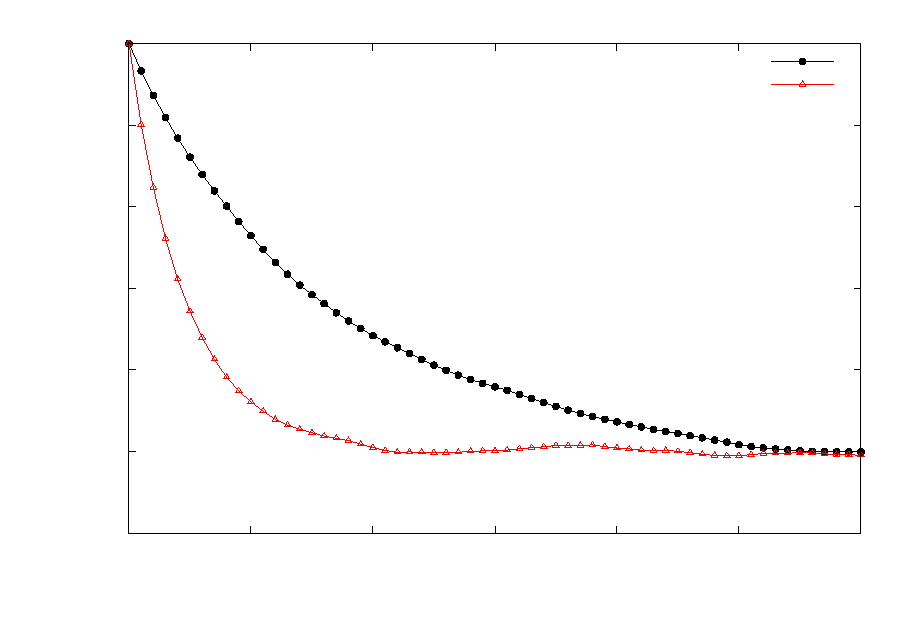
\includegraphics{autocorrelationzoomedin}}%
    \gplfronttext
  \end{picture}%
\endgroup

	\caption{Autocorrelation of the square of the magnetization}
	\label{fig:autocorrelation}
\end{figure}

%\subsection{Simulation at the finest level}
%compare result of m, $m^2$, e to expectation
%
%\subsection{Simulation of the Multigrid-algorithm}
%\paragraph{$\gamma=1$}
%plot autocorrelation
%compare result of m, $m^2$, e to expectation
%\paragraph{$\gamma=2$}
%plot autocorrelation
%compare result of m, $m^2$, e to expectation

\newpage	
\listoffigures
\listoftables
\printbibliography
\end{document}
